\documentclass[times, utf8, zavrsni]{fer}
\usepackage{booktabs}


\usepackage[croatian]{babel} 
\usepackage{amssymb}
\usepackage{amsmath}
\usepackage{txfonts}
\usepackage{mathdots}
\usepackage{titlesec}
\usepackage{array}
\usepackage{lastpage}
\usepackage{etoolbox}
\usepackage{tabularray}
\usepackage{color, colortbl}
\usepackage{adjustbox}
\usepackage{geometry}
\usepackage[classicReIm]{kpfonts}
\usepackage{hyperref}
\usepackage{fancyhdr}
\usepackage[T1]{fontenc}     % default is 'OT1'
\usepackage[utf8]{inputenc}
\usepackage{graphicx}

\usepackage{float}
\usepackage{setspace}
\restylefloat{table}


%boja za privatni i udaljeni kljuc u tablicama
\definecolor{LightBlue}{rgb}{0.9,0.9,1}
\definecolor{LightGreen}{rgb}{0.9,1,0.9}

%Promjena teksta za dugačke tablice
\DefTblrTemplate{contfoot-text}{normal}{Nastavljeno na idućoj stranici}
\SetTblrTemplate{contfoot-text}{normal}
\DefTblrTemplate{conthead-text}{normal}{(Nastavljeno)}
\SetTblrTemplate{conthead-text}{normal}
\DefTblrTemplate{middlehead,lasthead}{normal}{Nastavljeno od prethodne stranice}
\SetTblrTemplate{middlehead,lasthead}{normal}




\begin{document}

% TODO: Navedite broj rada.
\thesisnumber{663}

% TODO: Navedite naslov rada.
\title{Mobilna igra za vježbanje matematike}

% TODO: Navedite vaše ime i prezime.
\author{Denis Pipalović}

\maketitle

% Ispis stranice s napomenom o umetanju izvornika rada. Uklonite naredbu \izvornik ako želite izbaciti tu stranicu.
\izvornik

% Dodavanje zahvale ili prazne stranice. Ako ne želite dodati zahvalu, naredbu ostavite radi prazne stranice.
\zahvala{}

\tableofcontents

\chapter{Uvod}
	Matematika, osim što je predmet koji se predaje u svim razredima osnovnih i srednjih škola, također je i znanost iz područja prirodnih znanosti.
Značaj matematike vidljiv je ne samo u drugim poljima područja prirodnih znanosti, već i u svim drugim područjima, posebice u području tehničkih znanosti.
Ne poznavanje osnova matematike negativno se odražava na učenikove školske uspjehe kroz cijelo školovanje. Jedan od problema svakako je problem pristupa nastavnika
 u učenju matematike, odnosno manjak povlačenja paralela sa stvarnim svijetom i pokazivanja primjena matematike; ovakav pristup demotivira učenika u vježbanju matematike
i savladavanju čak i osnovnih računskih operacija. Jednom izgubljenu motivaciju za neko područje teško je vratiti nazad.

Primjenom gamifikacije u edukaciji učenicima bi se razne teme i ishodi učenja mogle prezentirati kroz zanimljive načine, samim time i povećati zainteresiranost za nekom temom 
ili predmetom. S obzirom na to da djeca u novije doba koriste pametne uređaje sve više i više, gamifikacija jedan od način kroz koji bi to vrijeme na mobitelu moglo biti potrošeno
 u edukativne svrhe; kroz zabavu!

S obzirom na navedeno, tema ovog rada je napraviti mobilnu igru za vježbanje matematike u nižim razredima osnovne škole koja će kroz zanimljiv i interaktivan način pružati  ugodnije iskustvo
vježbanja matematičkih zadataka. Igra je zamišljena kao tzv. „endless runner“ u kojoj igrač skuplja padajuće objekte ovisno o trenutnom zadatku (npr. samo parne brojeve, brojeve veće od zadanog,
brojeve djeljive s određenim brojem, samo kvadrate i slično) i sakuplja bodove. Kako igra ne bi postala monotona kroz kratko vrijeme igranja cilj je napraviti da igra postaje progresivno sve teža
i teža, no do te mjere da se ne postigne negativan efekt u drugom ekstremu; igra ne smije postati niti previše teška jer bi samim time postala i demotivirajuća! Stoga je cilj da se težina igre
dinamički prilagođava mogućnostima učenika. Osim same mobilne igre, potrebno je izgraditi i jednostavno web sučelje za učitelja kako bi mogao postavljati tipove zadataka koji prate temu onoga što
se trenutno predaje na nastavi. Kroz navedeno web sučelje nastavniku će se pružati i mogućnost pregleda rezultata pojedinog učenika te uvid u detalje igre kao što je tip zadatak na kojem je učenik 
griješio, ukupno vrijeme igranja i slično. Kako bi igra bila dostupna svima koji ju požele igrati, odnosno kako igra ne bi ovisila o postavkama učitelja, postojati će i zadane postavke koje će se moći
 prilagođavati kroz postavke same igre. 



\chapter{Naslov 1}
Poglavlje 1

\section{Introduction}
Podpoglavlje 1.1

\section{Introduction}
Podpoglavlje 1.2

\chapter{Naslov2}
Poglavlje 2



\chapter{Baza podataka}
	Baze podataka su organizirane kolekcija podataka koje omogućavaju laki pristup podacima, uređivanje podataka i upravljanje istih. U sklopu ovog projekta koristio se
	SQL tip baze podataka, konkretnije PostgreSQL. PostgreSQL je besplatni, open-source sustav za upravljanje bazom podataka (SUBP) iza kojeg je više od 30 godina aktivnog razvoja.
	
	
	\section{ER dijagram}
		Sljedeća slika prikazuje ER dijagram baze podataka.
		\begin{figure}[H]
			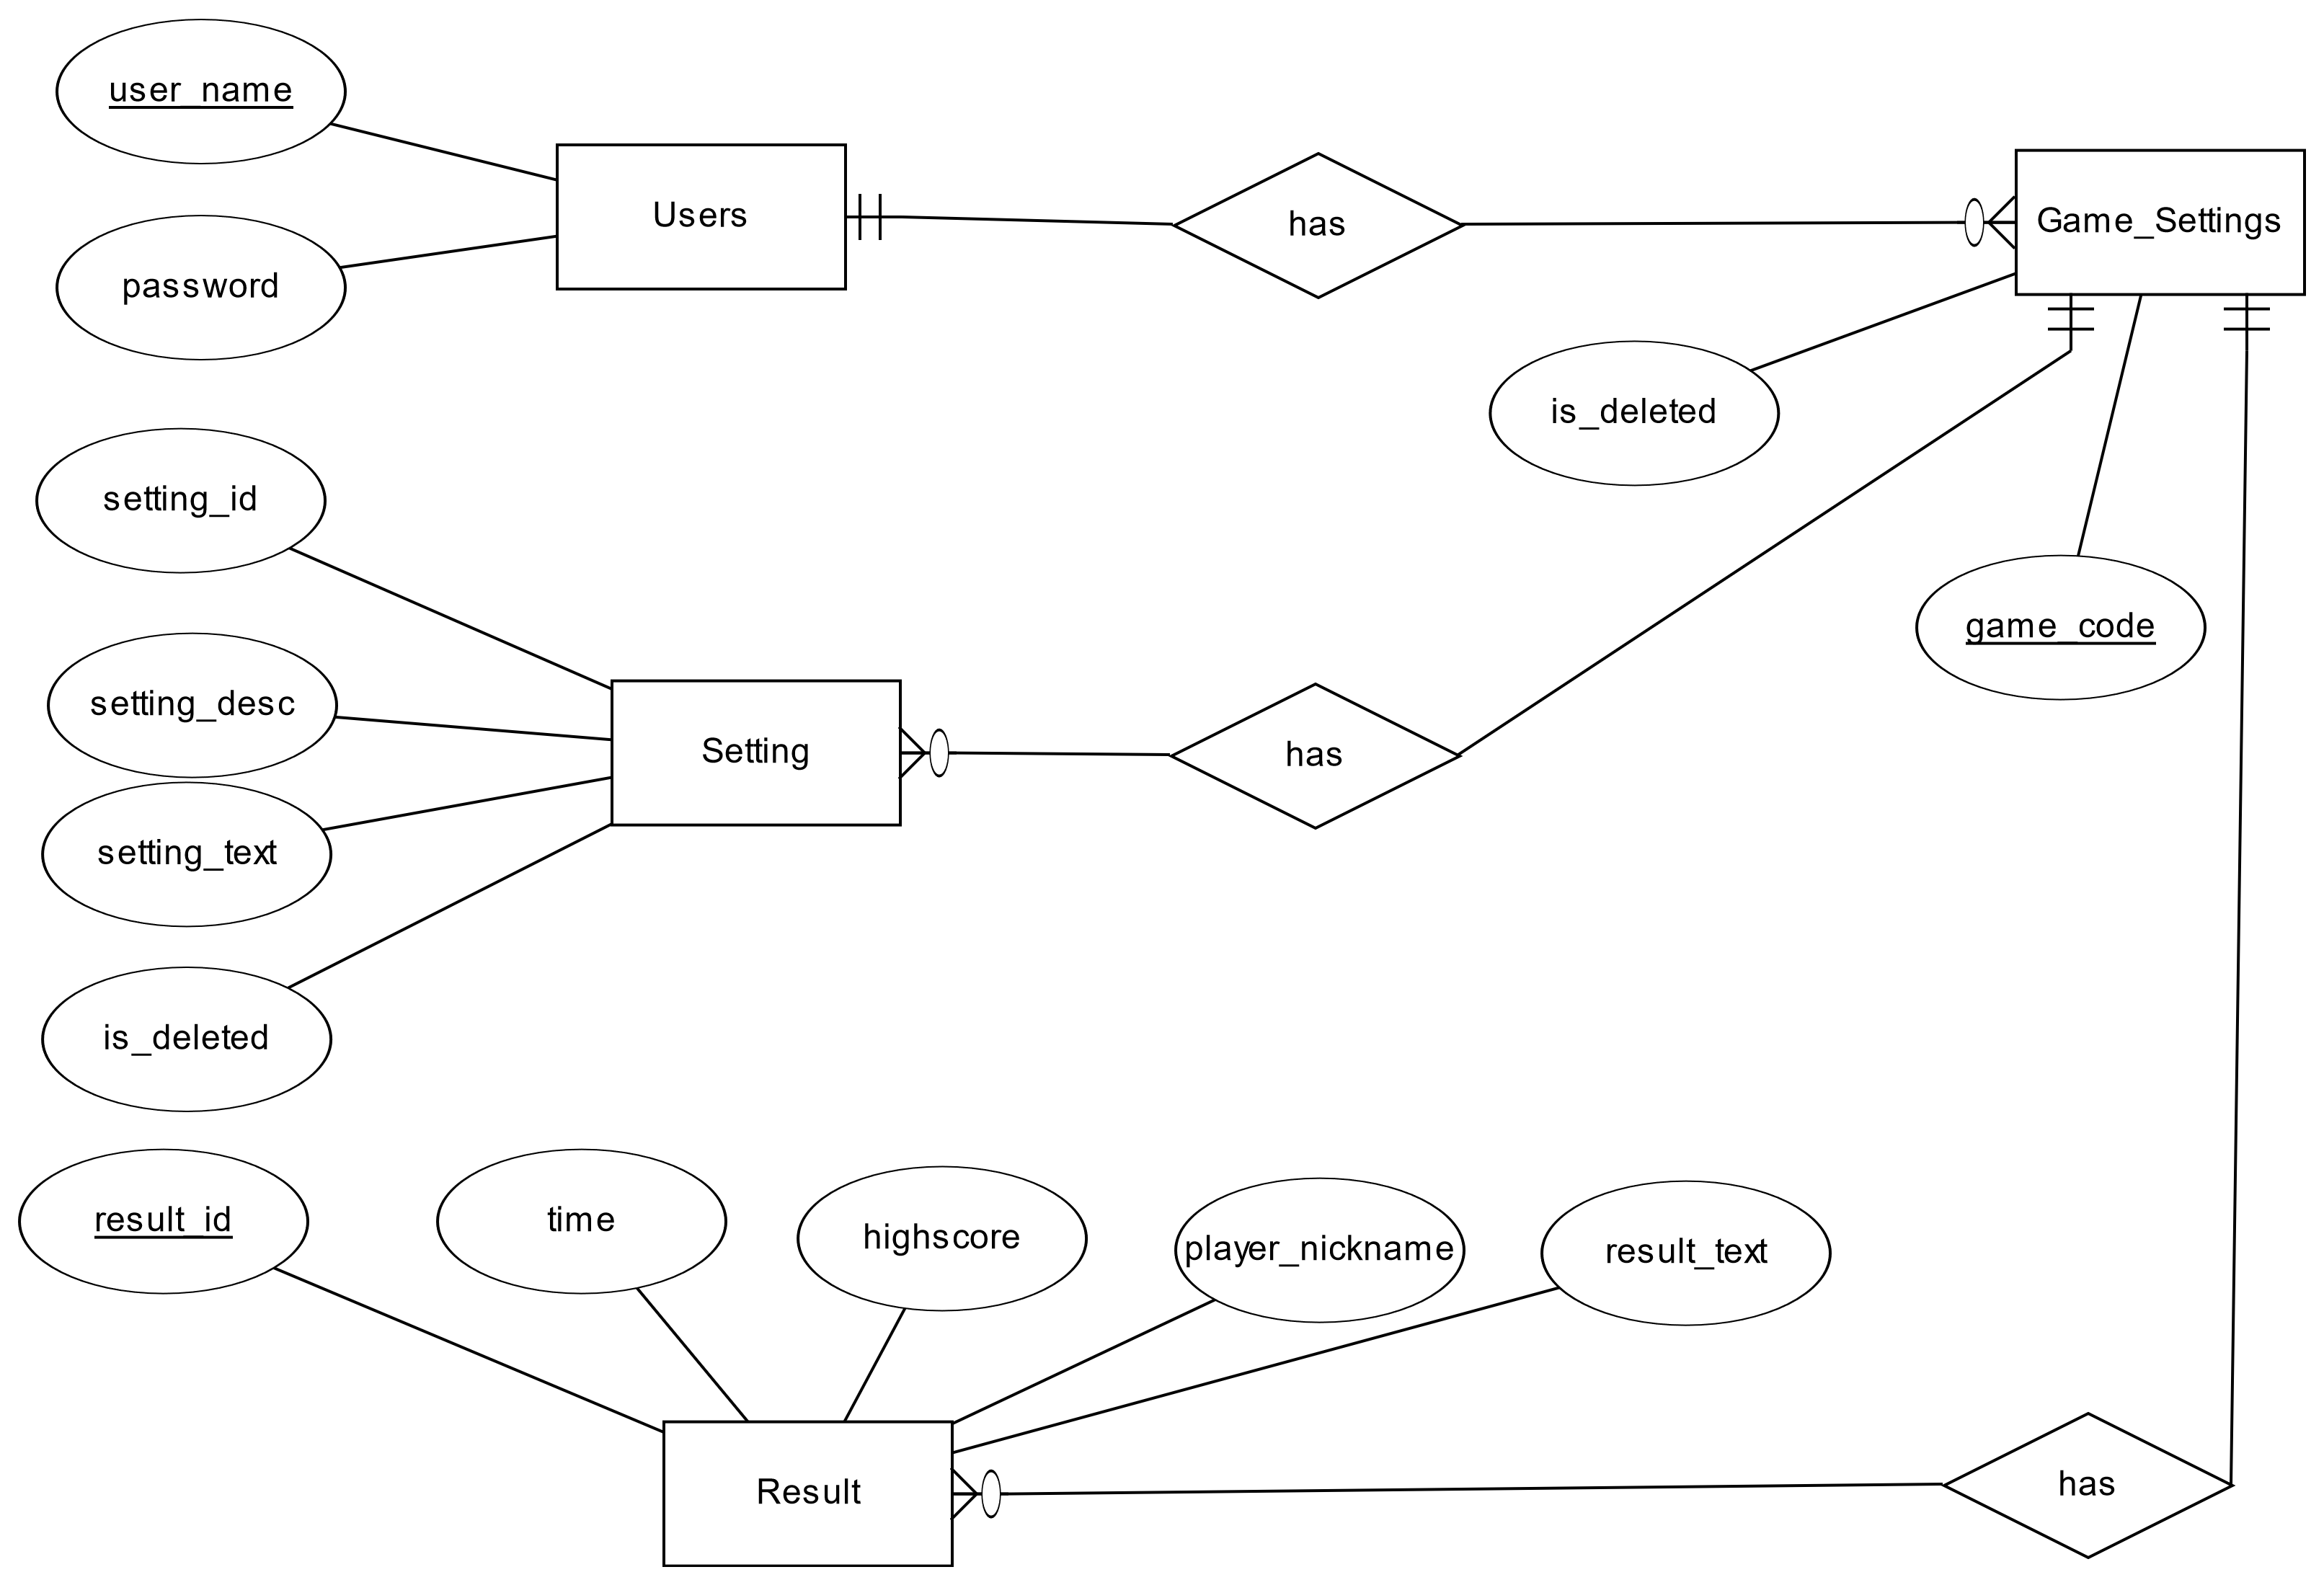
\includegraphics[width=\linewidth]{"slike/ER.png"} 
			\centering
			\caption{ER dijagram baze podataka}
			\label{fig:erdijagram}
		\end{figure}

	
	\section{Opis entiteta i tablica}
			\textbf {Users} \hspace{5mm}
			{Ovaj entitet označava korisnika koji koristi web aplikaciju, odnosno web sučelje za učitelja. Sadrži atribute: user\_ name i password.
			Atribut user\_ name predstavlja korisničko ime korisnika, dok atribut password označava zaporku koja se ne sprema u "plain-textu", već kao 
			rezultat hash funkcije.
			Ovaj entitet u vezi je \textit{One-To-Many} s entitetom Game\_ Settings preko atributa user\_name.}
				
				\begin{longtblr}[
					label=none,
					entry=none
					]{
						width = \textwidth,
						colspec={|X[6,l]|X[6, l]|X[20, l]|}, 
						rowhead = 1,
					} %definicija širine tablice, širine stupaca, poravnanje i broja redaka naslova tablice
					\hline \multicolumn{3}{|c|}{\textbf{Users}}	 \\ \hline[3pt]
					\SetCell{LightGreen}user\_name & VARCHAR	&  	jedinstveni naziv korisnika  	\\ \hline
					password	& VARCHAR &  rezultat hash funkcije nad zaporkom 	\\ \hline 
				\end{longtblr}



			\textbf {Game\_ Settings} \hspace{5mm}
			{Ovaj entitet označava jedan "game room". Sadrži atribute: game\_ code i is\_ deleted.
			Ovaj entitet u vezi je \textit{Many-To-One} s entitetom Users preko atributa user\_ name, u vezi \textit{One-To-Many} s
			entitetom Setting preko atributa game\_ code te u vezi \textit{One-To-Many} s entitetom Result preko atributa game\_ code.}
				
				\begin{longtblr}[
					label=none,
					entry=none
					]{
						width = \textwidth,
						colspec={|X[6,l]|X[6, l]|X[20, l]|}, 
						rowhead = 1,
					} 
					\hline \multicolumn{3}{|c|}{\textbf{Game\_ Settings}}	 \\ \hline[3pt]
					\SetCell{LightGreen}game\_ code & INT	&  	jedinstveni idenfitikator game\_ settings   	\\ \hline
					is\_ deleted & INT & zastavica koja govori jesu li "game room" obrisan \\ \hline
					\SetCell{LightBlue}user\_ name & VARCHAR & oznaka korisnika kojem "game room" pripada \\ \hline
				\end{longtblr}


			\textbf {Setting} \hspace{5mm}
			{Ovaj entitet označava jedanu postavku. Sadrži atribute: setting\_ id, setting\_ desc, setting\_ text i is\_ deleted.
			Ovaj entitet u vezi je \textit{Many-To-One} s entitetom Game\_ Settings preko atributa game\_ code.}
				
				\begin{longtblr}[
					label=none,
					entry=none
					]{
						width = \textwidth,
						colspec={|X[6,l]|X[6, l]|X[20, l]|}, 
						rowhead = 1,
					} 
					\hline \multicolumn{3}{|c|}{\textbf{Setting}}	 \\ \hline[3pt]
					\SetCell{LightGreen}setting\_ id & INT	&  	jedinstveni idenfitikator za Setting  	\\ \hline
					setting\_desc & VARCHAR & tekst koji opisuje cilj zadatka \\ \hline
					setting\_text & VARCHAR & postavka formatirana tako da bude razumljiva mobilnoj igri \\ \hline
					is\_ deleted & INT & zastavica koja govori je li postavka obrisana \\ \hline
					\SetCell{LightBlue}game\_code & INT & oznaka Game\_Settings kojem Setting pripada \\ \hline
					
				\end{longtblr}
				
			
			\textbf {Result} \hspace{5mm}
			{Ovaj entitet označava jedan rezultat igranja igre na mobitelu uz preuzete postavke.
			Sadrži atribute: result\_ id, time, highscore, player\_ nickname te result\_ text.
			Ovaj entitet u vezi je \textit{Many-To-One} s entitetom Game\_ Settings preko atributa game\_ code.}
				
				\begin{longtblr}[
					label=none,
					entry=none
					]{
						width = \textwidth,
						colspec={|X[6,l]|X[6, l]|X[20, l]|}, 
						rowhead = 1,
					} 
					\hline \multicolumn{3}{|c|}{\textbf{Result}}	 \\ \hline[3pt]
					\SetCell{LightGreen}result\_ id & INT	&  	jedinstveni idenfitikator za Result  	\\ \hline
					time & VARCHAR & vrijeme pohrane rezultata u bazu podatka \\ \hline
					highscore & VARCHAR & ostvareni rezultat na igri  \\ \hline
					player\_ nickname & VARCHAR & nadimak igrača  \\ \hline
					result\_text & VARCHAR & JSON polje s događajima igre  \\ \hline
					\SetCell{LightBlue}game\_code & INT & oznaka Game\_Settings kojem Result pripada \\ \hline
					
				\end{longtblr}

	\newpage
	\section{Relacijski dijagram}
		Sljedeća slika prikazuje relacijski dijagram baze podataka.
		\begin{figure}[H]
			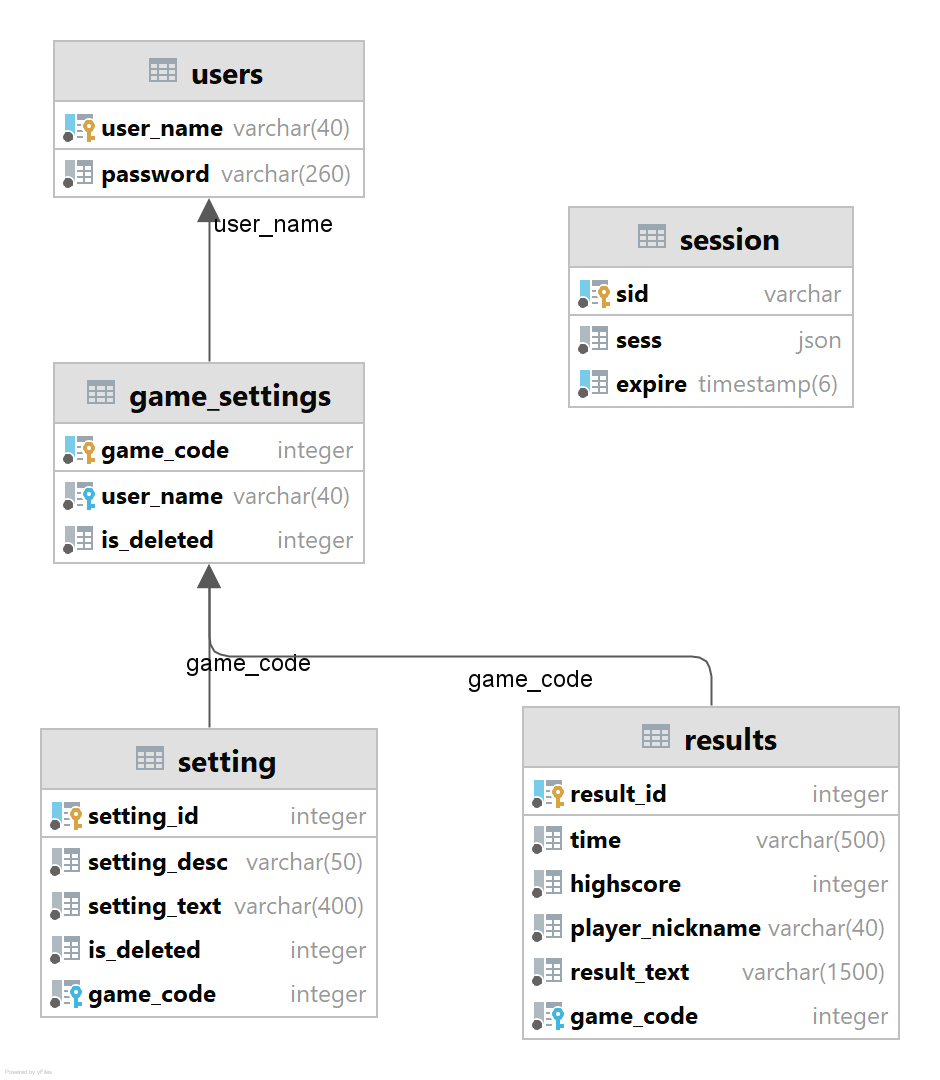
\includegraphics[width=\linewidth]{"slike/REL.png"} 
			\centering
			\caption{Relacijska shema baze podataka}
			\label{fig:relshema}
		\end{figure}


\chapter{Naslov 4}
Poglavlje 4

\bibliography{literatura}
\bibliographystyle{fer}

\begin{sazetak}
Sažetak na hrvatskom jeziku.

\kljucnerijeci{Ključne riječi, odvojene zarezima.}
\end{sazetak}

% TODO: Navedite naslov na engleskom jeziku.
\engtitle{Mobile game for practicing math}
\begin{abstract}
Abstract.

\keywords{Keywords.}
\end{abstract}

\end{document}
